Designet af robotten for dette projekt er yderst vigtigt; det er grundstenen i projektet, og uden en velfungerende robot (og specifikt kontrol af denne), vil det blive yderst svært at løse problemstillingen for projektet tilfredsstillende.
At navigere et ukendt areal med en kendt position kræver præcis kontrol af enhver bevægelse, hvorfor dette afsnit fokuserer på hvordan vi er kommet frem til designet af den endelige robot, samt hvilke særlige problemstillinger der ligger til grund for designet.

\section{Design overvejelser}
Designet af robotten har været en del af læringsprocessen for hvordan man bygger en robot af \lego NXT komponenterne, hvorfor design processen kan ses som en iterativ process, hvor designet er blevet radikalt ændret for hver iteration, indtil et tilfredsstillende resultat er opnået.

%Da vi fik udleveret \lego var førsteprioriteten at få bygget en \textit{kørende} robot, således vi kunne begynde at lave små programmer til den for at undersøge hvordan den kan styres.


\paragraph{Første design} af robotten var meget simpelt, hvor selve NXT enheden fungerede som dens \textit{base}.
På denne var alle andre komponenter monteret, hvilket var uhensigtsmæssigt i forhold til den videre udvikling af robotten.
F.eks. vanskeliggjorde det at finde en god placering af robottens ultrasoniske sensor.
Derfor blev det besluttet at droppe dette design.

\paragraph{Andet design} var en delvis videreudvikling af det første design; men denne gang var konstruktionen blevet ændret for at få plads til en ultrasonisk sensor foran -- sammen med en motor til at rotere den med.
Igen viste designet sig at være for simpelt, men denne gang var det i forhold til styringen af sensoren.
Problemet ligger i at sensoren var monteret i 1:1 forhold mellem motoren der roterer den, hvilket gav alt for store usikkerheder når sensoren skulle roteres x-antal grader (ofte mere end 5\degree).
Dette skyldes de usikkerheder der er forbundet med styringen af motoren samt slid af dens interne komponenter, hvilke vores test også beskriver i .\thilemann{indsæt kilde til test her...}

\paragraph{Design krav}
Disse to design ledte frem til følgende krav til det endelige design af robotten:

\begin{itemize}
\item Den ultrasoniske sensor skal kunne styres til højst 1\degree~nøjagtighed, med en foreslået gearing på 1:4.
\item Sensoren(e) skal kunne foretage en 360\degree~måling.
\item Sekundært indføres der en gearing af hjulene for bedre styring af robotten (nedgearing for højere moment).
\item Mere stabil opbygning for at mindske generelle usikkerheder.
\end{itemize} 


\section{Endeligt design}
Udgangspunktet for det endelige design er udelukket baseret på ovenstående design krav. 


\begin{figure}
\centering
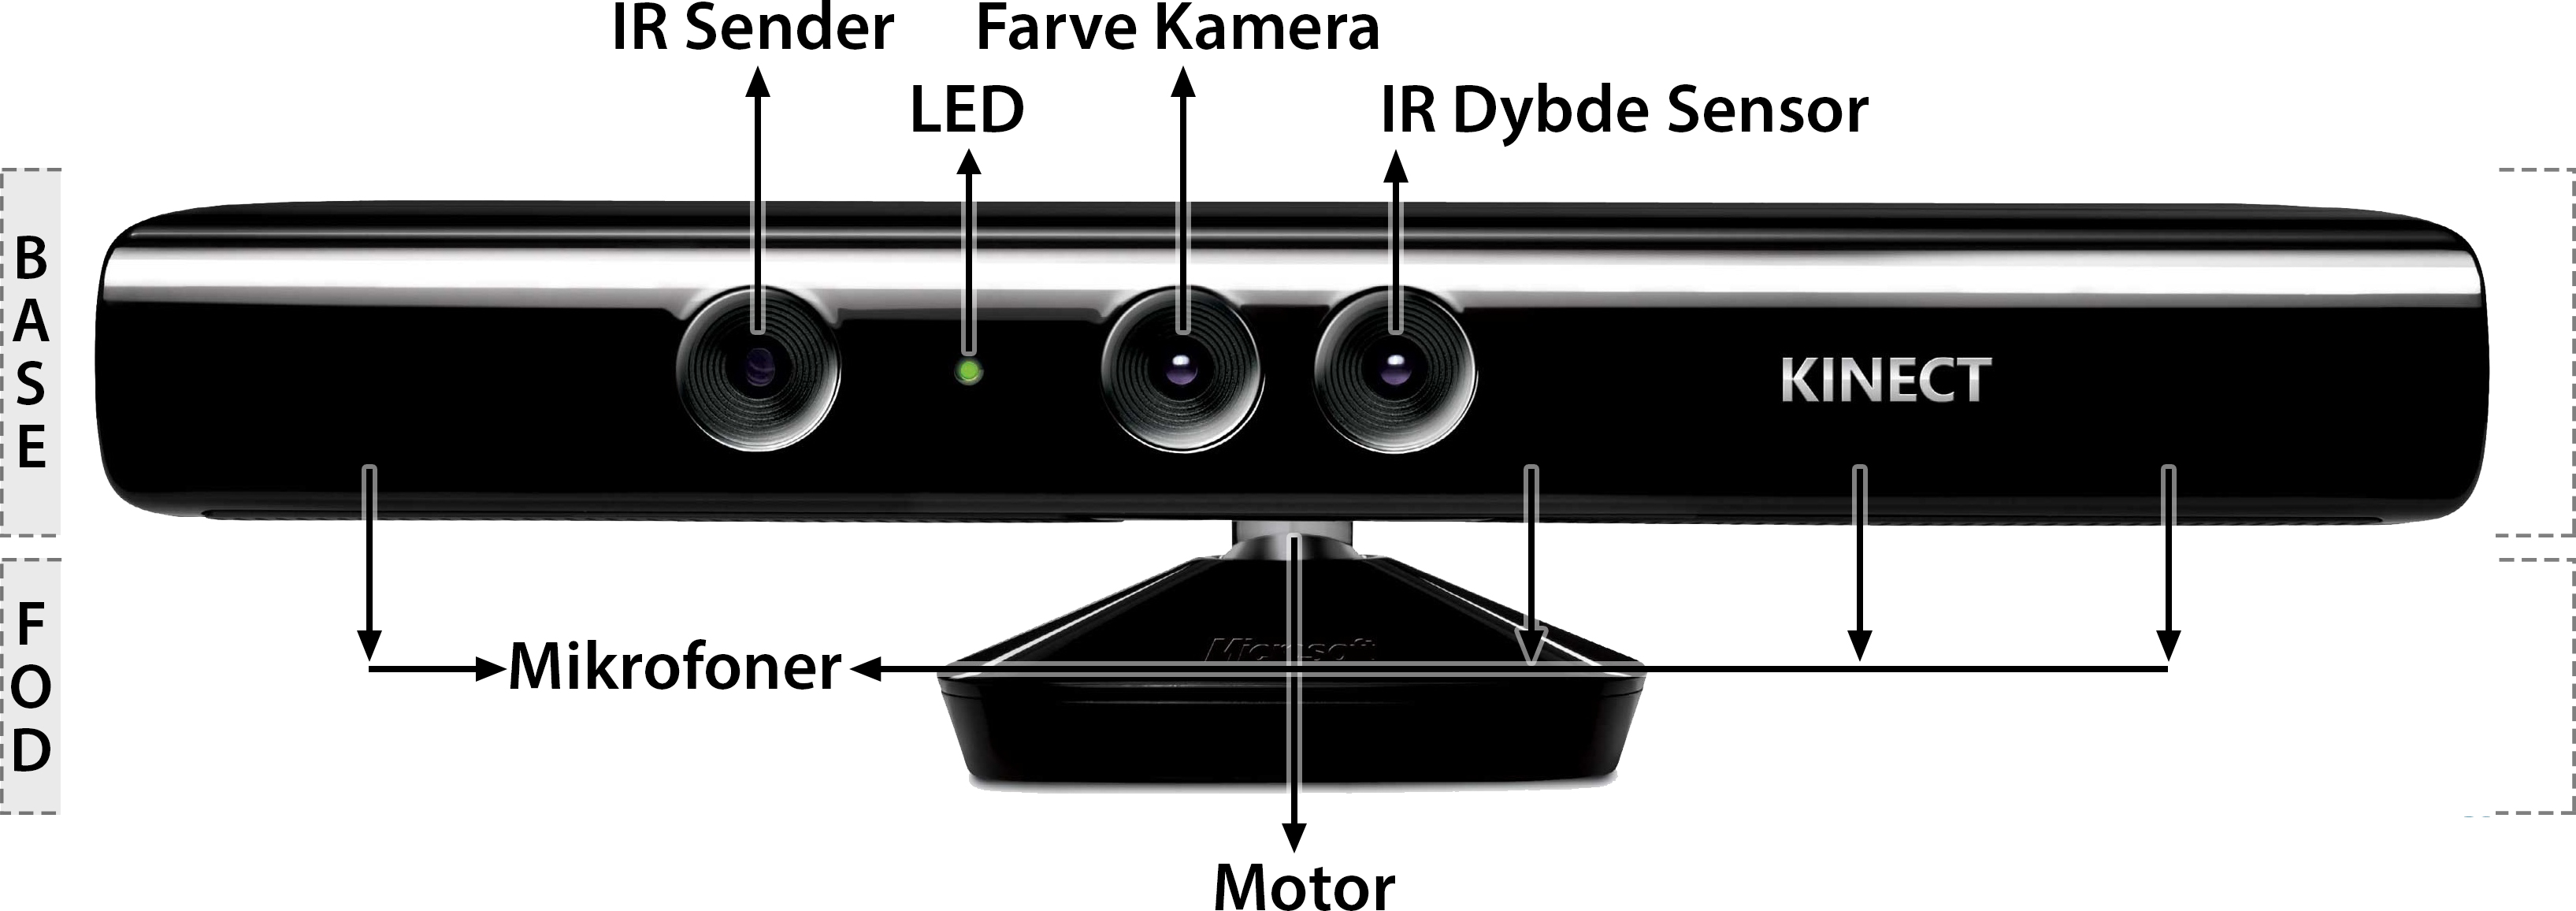
\includegraphics[width=0.5\textwidth]{kinect/kinect}
\caption{Endelige design af vores robot.}
\label{robot:opbygning}
\end{figure}

\subsection{Komponenters placering}
test

\paragraph{Basen}
test

\paragraph{Fremdrift}
- valg af hjul og fremdrift
- grund til gearing

\paragraph{Sensorer}
- sensorens placering og mobilitet
